%%%%%%%%%%%%%%%%%%%%%%%%%%%%%%%%%%%%%%%%%%%%%%%%%%%%%%%%%%%%%%%%%%%%%%%%%%%%%%%%%%%%%%%%%%%%%%%%%%%%%%%%%%%%%%%%%%%%%%%%
\newpage
\chapter {\Large{Siminov Initialization}}

\section{Siminov Native ORM Framework}
Every native application when it starts they need to first initialize Siminov Native ORM. They can do this by invoking initialize method of siminov.orm.Siminov class by passing \textbf{ApplicationContext} object as paramter to method.

		\begin{center}
			\colorbox{grey}{
				\parbox[t]{.8\linewidth}{
					\fontsize{11pt}{11pt}\selectfont % The first argument for fontsize is the font size of the text and the second is the line spacing - you may need to play with these for your particular title
					\vspace*{0.1cm} % Space between the start of the title and the top of the grey box
		
					\hfill \textbf{Note} \\

					Use Siminov Native ORM only if you are buiding Android Native based application. 

					\vspace*{0.0cm} % Space between the end of the title and the bottom of the grey box
				}
			}

		\end{center}



\par
There are two ways to initialize Siminov Native ORM

\begin{enumerate}

	\item \small \textbf{Initializing Siminov Native ORM From Sub-Class Of Application}

		\lstinputlisting[language=Java]{Resources/siminov_native_orm_initialization_example_1.txt}
	
		\begin{center}
			\colorbox{grey}{
				\parbox[t]{.8\linewidth}{
					\fontsize{11pt}{11pt}\selectfont % The first argument for fontsize is the font size of the text and the second is the line spacing - you may need to play with these for your particular title
					\vspace*{0.1cm} % Space between the start of the title and the top of the grey box
		
					\hfill \textbf{Note} \\

					Android provides support in every application to create an application wide class. The base class for this is the android.app.Application class. 

					\vspace*{0.0cm} % Space between the end of the title and the bottom of the grey box
				}
			}

		\end{center}

	\item \small \textbf{Initializing Siminov Native ORM From Sub-Class Of Activity}

		\lstinputlisting[language=Java]{Resources/siminov_native_orm_initialization_example_2.txt}


		\begin{center}
			\colorbox{grey}{
				\parbox[t]{.8\linewidth}{
					\fontsize{11pt}{11pt}\selectfont % The first argument for fontsize is the font size of the text and the second is the line spacing - you may need to play with these for your particular title
					\vspace*{0.1cm} % Space between the start of the title and the top of the grey box
		
					\hfill \textbf{Note} \\

					If you are initializing Siminov Native ORM from activity sub class then you should pass application context not the activity context. See above example.

					\vspace*{0.0cm} % Space between the end of the title and the bottom of the grey box
				}
			}

		\end{center}


\end{enumerate}



		\begin{center}
			\colorbox{grey}{
				\parbox[t]{.8\linewidth}{
					\fontsize{11pt}{11pt}\selectfont % The first argument for fontsize is the font size of the text and the second is the line spacing - you may need to play with these for your particular title
					\vspace*{0.1cm} % Space between the start of the title and the top of the grey box
		
					\hfill \textbf{Note} \\

					\begin{enumerate}

						\item \small Application should call siminov.orm.Siminov initialize only once in the life time of application.

						\item \small Once Siminov Native ORM is initialized it can not be re initialized.

					\end{enumerate}

					\vspace*{0.0cm} % Space between the end of the title and the bottom of the grey box
				}
			}

		\end{center}


\par
\textbf{Steps performed in initializating Siminov Native ORM Framework}

	\begin{enumerate}

		\item \small \textbf{Database Creation}: Siminov provides \textbf{Initialization Layer} which handles the creation of databases required by application. 

		\par
		Siminov Native ORM follows below steps to create databases required by application.

		\begin{enumerate}

			\item \small \textbf{Step 1}: Then application invokes initialize method, it checks wheather database exists or not.

			\item \small \textbf{Step 2}: If application database does not exists, Siminov Native ORM will create database required by the application.

			\item \small \textbf{Step 3}: If application database exists, then it will read all desriptors defined by application based on load\_initially property defined in ApplicationDescriptor.si.xml file.

		\end{enumerate}

		
		\item \small \textbf{Initialize Resources Layer}	: Any resource created by Siminov Native ORM Framework is places in resource layer of Siminov Native ORM. You can use API's provided by Resources class to get required object.
			
			\lstinputlisting[language=java]{Resources/resources_class_apis.txt}


	\end{enumerate}



\section{Siminov Hybrid Framework}

Hybrid application is a combination of Native and Web. Siminov Hybrid Framework is build over Siminov Native ORM, therefore it provides both Web ORM as well as Native ORM features.

	
		\begin{center}
			\colorbox{grey}{
				\parbox[t]{.8\linewidth}{
					\fontsize{11pt}{11pt}\selectfont % The first argument for fontsize is the font size of the text and the second is the line spacing - you may need to play with these for your particular title
					\vspace*{0.1cm} % Space between the start of the title and the top of the grey box
		
					\hfill \textbf{Note} \\
					If you are using Siminov Hybrid Framework then you dont have to explicitly initialize Siminov Native ORM because Hybrid will take care of that.

					\vspace*{0.0cm} % Space between the end of the title and the bottom of the grey box
				}
			}

		\end{center}


Initializing Siminov Native Framework is a two way of initialization through Native and Web.


\begin{enumerate}

	\item \small \textbf{Intialize Siminov Hybrid From Native When Application Starts}
		
		Initialize Siminov Hybrid Framework by invoking initialize API of siminov.hybrid.Siminov class and provide ApplicationContext and WebView as a parameter to API. Internally Siminov Hybrid Framework will automatically initialize Siminov Native ORM.
		\lstinputlisting[language=Java]{Resources/siminov_hybrid_initialization_example_1.txt}

	\item \small \textbf{Initialize Siminov Hybrid From Web When Device Get Ready}
		
		Intialize Siminov Hybrid Framework by invoking initialize API of Siminov function, once Siminov gets initialized you will get a call back in firstTimeSiminovInitialized/siminovInitialized Event Handler.

		\lstinputlisting[language=Java]{Resources/siminov_hybrid_initialization_example_2.txt}
	
		\begin{center}
			\colorbox{grey}{
				\parbox[t]{.8\linewidth}{
					\fontsize{11pt}{11pt}\selectfont % The first argument for fontsize is the font size of the text and the second is the line spacing - you may need to play with these for your particular title
					\vspace*{0.1cm} % Space between the start of the title and the top of the grey box
		
					\hfill \textbf{Note} \\
					
						\begin{enumerate}
			
							\item \small If you use Siminov Hybrid Framework it is mandatory to register for Events.
			
							\item \small If you use only Siminov Native ORM it is not mandatory to register for Events.

						\end{enumerate}					



					\vspace*{0.0cm} % Space between the end of the title and the bottom of the grey box
				}
			}

		\end{center}


\end{enumerate}





\section{Lazy Initialization VS Initial Initialization}

Siminov Framework provides easy configuration property in ApplicationDescriptor.si.xml file through which application developer can significantly improve the performance of Siminov. 


\begin{enumerate}

	\item \small \textbf{load\_initially}: \textit{TRUE}/\textit{FALSE}, It is not mandatory field, and default value is FALSE.

		\par
		\textbf{Example:} Siminov Template Application Example.
		\begin{figure}[htbp]
			\centering
				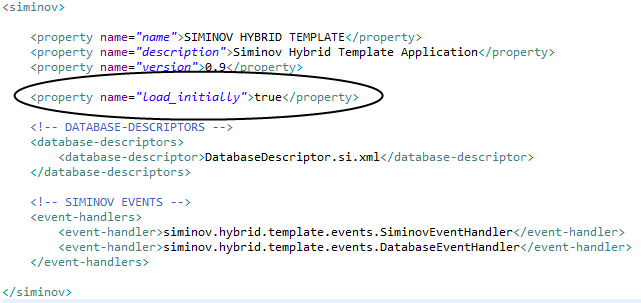
\includegraphics[height=5.6cm]{Resources/siminov_application_template_application_descriptor_load_example.png}
		\end{figure}

		\par
			Basically to map entity and database table, Siminov need DatabaseMappingDescriptor object which defines relation between entity and database table, this object is created by reading DatabaseMappingDescriptor.si.xml file defined by application.

		\par
			\textbf{Lazy Initialization (load\_initially=true)}: If load\_initially is set to true then Siminov will load all descriptors at time of Siminov initialization itself and will create all its corresponding DatabaseMappingDescriptor objects, and place them in resources layer of Siminov.

		\par
			\textbf{Initial Initialization (load\_initially=false)}: If load\_initially is set to false then Siminov will not load all descriptors at time of Siminov initialization. It will load descriptor only when it is required by Siminov.

\end{enumerate}


\newpage
\section{Handling Multiple Schema's}
Siminov framework supports multiple schema's if required by application. Basically each schema is defined using DatabaseDescriptor.si.xml file. You need to specify all DatabaseDescriptor.si.xml file path in ApplicationDescriptor.si.xml.

		\par
		\textbf{Example:} Siminov Template Application Example.
		\begin{figure}[htbp]
			\centering
				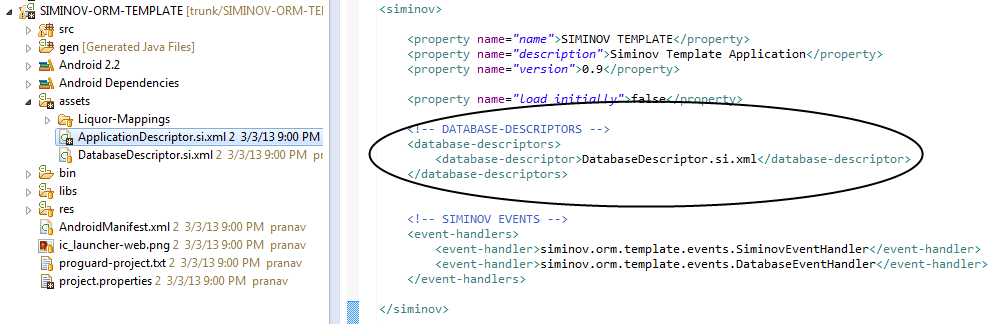
\includegraphics[height=5.8cm]{Resources/siminov_application_multiple_schemas_example.png}
		\end{figure}



